\section{Methodology}
\label{sec:-method}
\subsection{Crawler Operation}
The operation of the Tumblr crawler, affectionately referred to as ``the crawlblr,'' 
is described in the pseudocode in Fig. \ref{crawler}.  crawblr 
ran on a long-generic ACISS node with twelve cores, with 512 crawler 
instances and 200 database workers.  It operated in a 
depth-first-per-process manner, in order to guarantee that we 
established as complete a record as possible for the subset of Tumblr 
we surveyed. 
\begin{figure}
  \begin{algorithmic}[1]
    \Require usernames initialized with a well-connected user
    \Procedure{Crawl}{$usernames,usersseen,dbQ$}
    \While{usernames not empty}
    \State $user.1 \gets usernames.pop$
    \State $blog \gets open(user.1)$
    \State $user.2 \gets blog.postCount$
    \State $user.3 \gets blog.lastActive$
    \State $dbQ.push(user)$ \Comment{send user to database worker}
    \ForAll{posts in blog}
    \If{post is reblogged}
    \If{source not in usersseen}
    \State $usersseen.push(post.source)$
    \State $usernames.push(post.source)$
    \EndIf
    \State $Continue$\Comment{Go to next post}
    \ElsIf {post is original}
    \State $postOut.1 \gets user.1$
    \State $postOut.2 \gets post.id$
    \State $postOut.3 \gets post.type$
    \State $postOut.4 \gets post.timestamp$
    \State $postOut.5 \gets post.notecount$    
    \State $dbQ.push(postOut)$
    \ForAll{notes on post}
    \State $noteOut.1 \gets note.source$
    \State $noteOut.2 \gets note.via$
    \State $noteOut.3 \gets post.id$
    \State $noteOut.4 \gets note.type$
    \State $dbQ.push(noteOut)$
    \If{note.source not in usersseen}
    \State $usersseen.push(note.source)$
    \State $usernames.push(note.source)$
    \EndIf
    \If{note.via not in usersseen}
    \State $usersseen.push(note.via)$
    \State $usernames.push(note.via)$
    \EndIf
    \EndFor
    \EndIf
    \EndFor
    \EndWhile
    \State \textbf{return} $True$    
    \EndProcedure
    \Procedure{databaseWork}{$dbQ$}
    \While{dbQ not empty}
    \State $database.write(dbQ.pop)$
    \EndWhile
    \EndProcedure
  \end{algorithmic}
%%% Local Variables: 
%%% mode: latex
%%% TeX-master: "main"
%%% End: 

  \caption{Crawler operation}\label{crawler}
\end{figure}

As notes on a post are retained across reblogs, we defer the analysis 
of reblogged posts, by adding the source to the list of users to crawl.  
In so doing, we avoid double-counting, as post IDs are not retained 
across reblogs, preventing non-trivial uniqueness checking.

Users, notes, and pages are saved as tuples before being passed to a 
managed queue in shared memory.  The database worker pulls from this 
queue, and uses the cardinality of the tuples to discern which table 
in the SQLite database should take the information.  Each database 
process maintains a separate database, in order to parallelize the 
filesystem writes.  A separate program merges the databases together 
for analysis when crawlblr has finished.
\subsection{Database Arrangement}
\begin{figure*}
\centering
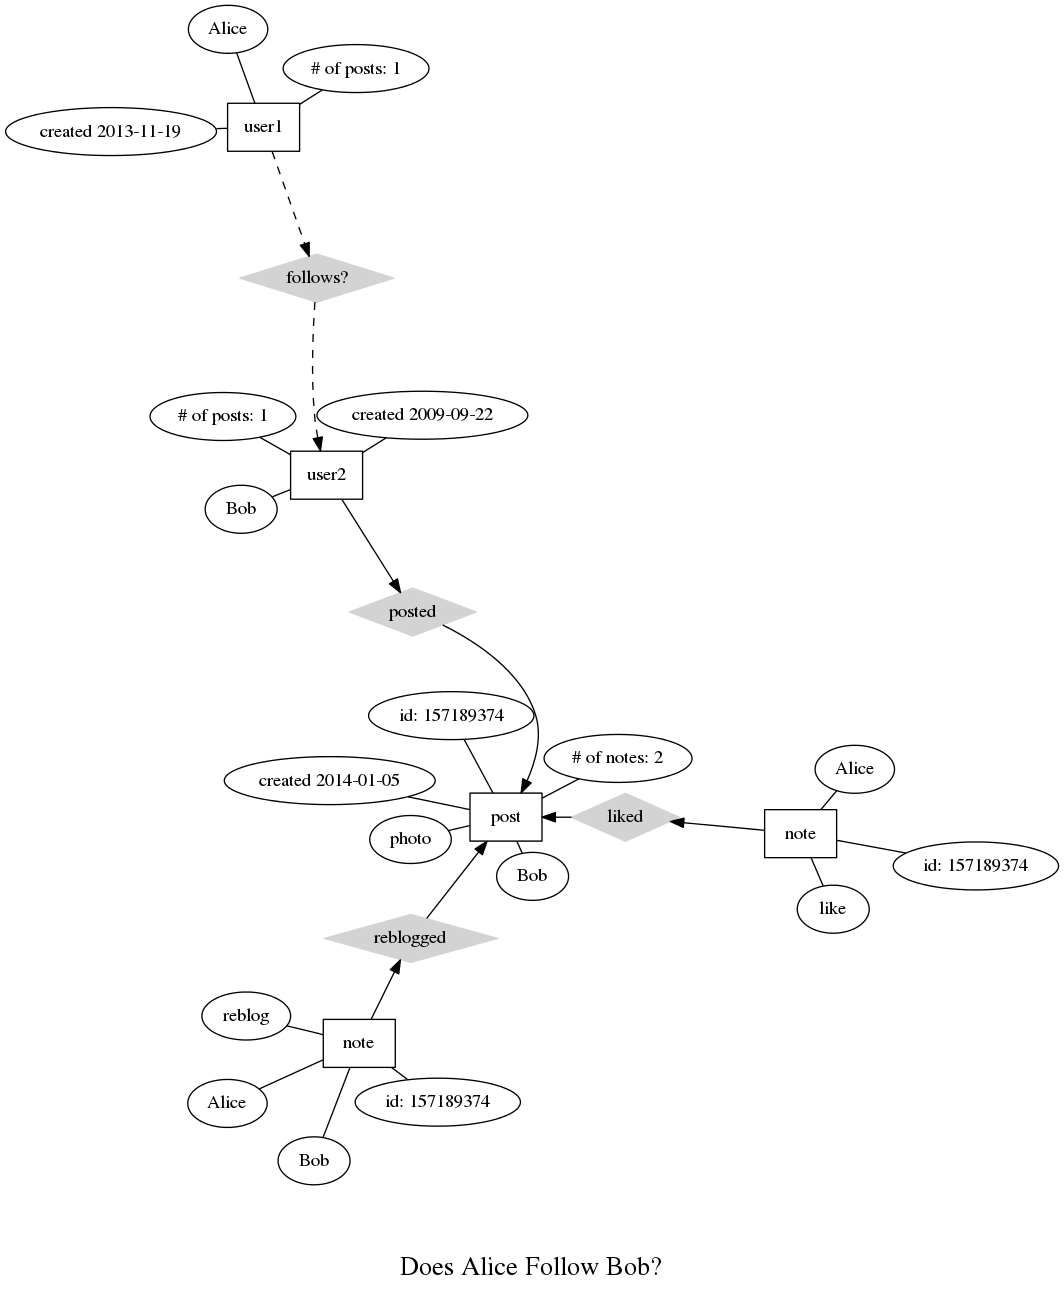
\includegraphics[width=\textwidth]{relations}
 \caption{Here we see a hypothetical relationship between two users}
 \label{fig:relations}
\end{figure*}

For each user, we logged their unique username, the number of posts 
they have contributed to Tumblr, and the date they joined. 

For each of those posts, we logged the unique post identifier, the 
date posted, the post type, and the number of notes.

Notes can take two forms: 

user likes content and 

user1, via user2, reblogs content.

We present the following logic as a technique for identifying potential 
links of the form user1 follows user2.

Likes and reblogs on reposts are conserved over all copies.  For likes, 
this means that a like on a reblog of content is indistinguishable from 
a like on the original piece of content itself, or a like on all 
separate instances of the content.
%%% Local Variables: 
%%% mode: latex
%%% TeX-master: "main"
%%% End: 
